\documentclass[letterpaper, 10pt]{article}
\usepackage{amsmath, bbm}
\usepackage{amssymb, amsthm}
%\usepackage{mathptmx}
%\usepackage[LY1]{fontenc}
\usepackage{fancyhdr}
\usepackage{graphicx}
\usepackage{subfigure}
\usepackage{verbatim}
\usepackage{array}
\usepackage{hyperref}
\usepackage[squaren]{SIunits}
\usepackage{color}

\topmargin 0in
\headheight 0.0pt

\headsep 0. in
%\bottommargin 1in
\oddsidemargin 0.0 in
\evensidemargin 0.0 in
\textwidth 6.5 in
\textheight 9 in

\renewcommand{\headrulewidth}{0pt}
\newcommand{\tmop}[1]{\operatorname{#1}}
\newtheorem{lemma}{Lemma}
\newtheorem{theorem}{Theorem}
\newtheorem{definition}{Definition}
\newtheorem{claim}{Claim}
\newtheorem{proposition}{Proposition}


\newcommand{\neal}[1]{\textcolor{red}{Neal: #1}}
\newtheorem{corollary}{Corollary}
\newtheorem{fact}{Fact}
%%%%%%%%%%%%%%%%%%%%%%%%%%%%%%%%%%%%%%
%%       EDIT THESE VARAIBLES       %%
%%%%%%%%%%%%%%%%%%%%%%%%%%%%%%%%%%%%%%


%%%%%%%%%%%%%%%%%%%%%%%%%%%%%%%%%%%%%
%%%%%%%%%%%%%%%%%%%%%%%%%%%%%%%%%%%%%%
    \newcommand\independent{\protect\mathpalette{\protect\independenT}{\perp}}
    \def\independenT#1#2{\mathrel{\setbox0\hbox{$#1#2$}%
    \copy0\kern-\wd0\mkern4mu\box0}} 
    \numberwithin{equation}{section} 
\author{Neal Wadhwa}
\title{AWGN in Motion Magnification}
\date{February 18, 2014}
\begin{document}
\newcommand{\D}{\mathcal{D}}
\newcommand{\pr}{\tmop{Pr}}
\newcommand{\R}{\mathbb{R}}
\newcommand{\beq}{\begin{equation}}
\newcommand{\eeq}{\end{equation}}
\newcommand{\E}{\mathbb{E}}
\newcommand{\Var}{\text{Var}}
\noindent
\maketitle
In this document, we assume a signal and noise model in which the motion signal has a decorrelation time greater than two frames (e.g. narrowband sinusoidal oscillations) and the noise is spatiotemporal IID additive Gaussian white noise in the image domain. We also assume that the video is mostly static, so that the noise is stationary in time. This noise model, while simple, illustrates the challenges of applying traditional LMMSE optimal techniques as the noise in the phase domain is nonstationary in space. The goal of this document is to provide a way to replace the temporal filter in our previous phase-based processing.
\begin{figure}[h]
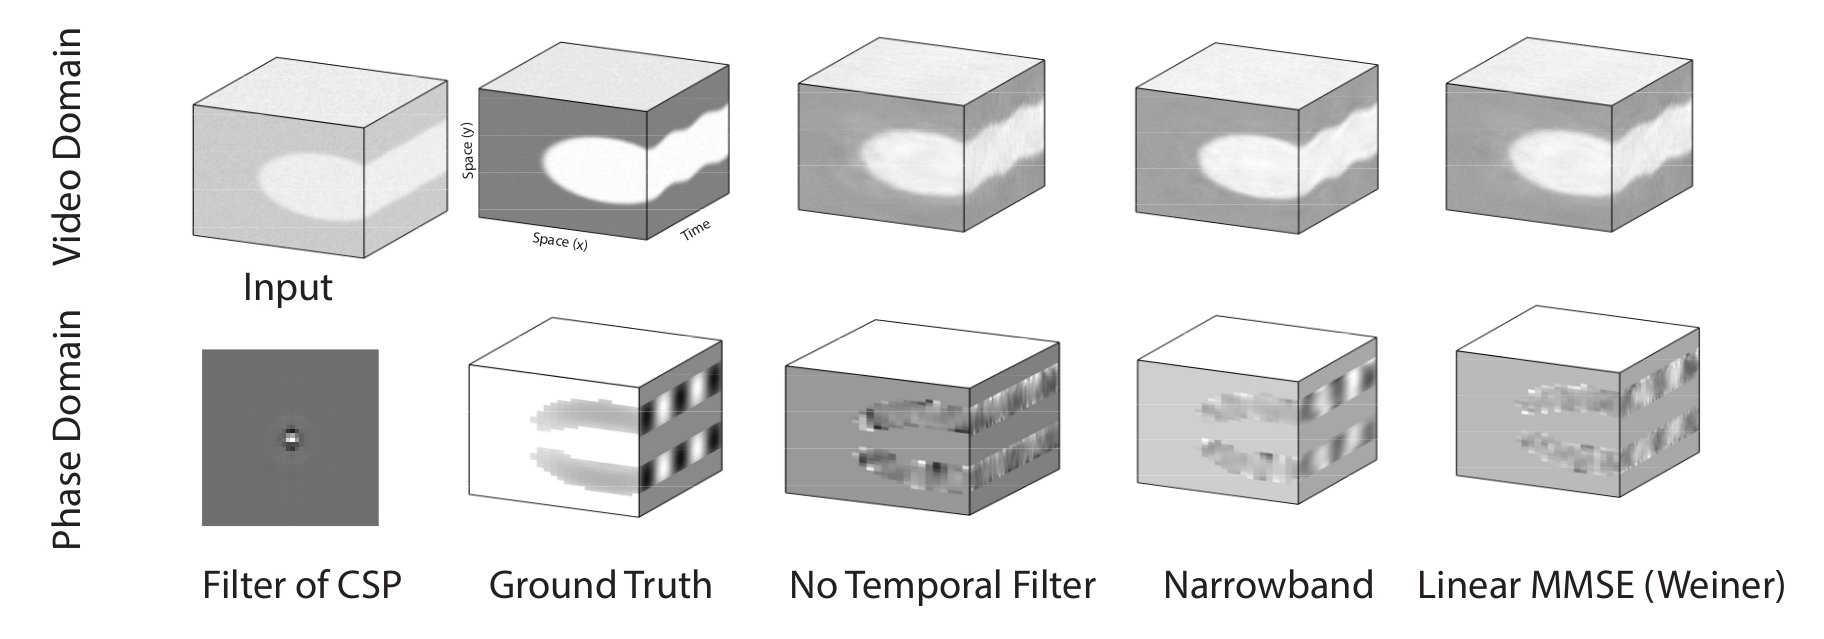
\includegraphics[width=\textwidth]{figPhaseModel01teaser/teaser.png}
\caption{Our technique applied to a synthetic disk oscillating vertically. The phase signal in one level of the pyramid is shown in the bottom row. We compare our technique to no temporal filtering and to manually tuned narrowband temporal filtering.}
\label{fig:teaser}
\end{figure}

\section{Noise Model}

\paragraph{AWGN in the Phase Domain}
In the phase domain, AWGN translates to approximately Gaussian white noise when the complex steerable pyramid coefficient has high amplitude. We show in this section that Gaussian noise is a good approximation to what the noise actually looks like. In a previous document, we showed that the phase signal has distribution 
\beq \mathcal{P}_{A_0,\theta_0}(\theta) = \frac{1}{2\pi} \text{exp}\left[-\frac{\beta^2\sin^2(\theta-\theta_0)}{2} \right]\left(\text{exp}\left[-\frac{\beta^2\cos^2(\theta-\theta_0)}{2}\right]+\beta\cos(\theta-\theta_0)\sqrt{\frac{\pi}{2}}\left(1+\text{erf}\left(\frac{\beta\cos(\theta-\theta_0)}{\sqrt{2}} \right)\right)\right) \label{eq:noisePDF01}\eeq
where $\beta$ is the amplitude to noise ratio. If we make the assumption that $\beta >>1$, that is the amplitude is much larger than the image noise, we can approximate Eq.~\ref{eq:noisePDF01} as
\beq \frac{\beta}{\sqrt{2\pi}} e^{-\frac{\beta^2(\theta-\theta_0)^2}{2}}\eeq
which is Gaussian. This breaks down when $\beta<<1$. By assuming the noise is Gaussian, we will overestimate the variance and downweight low amplitude points more than we should. However, I doubt this will make a huge difference as these points are typically so unreliable that they are already downweighted substantially.
\begin{figure}
\begin{tabular}{cccc}
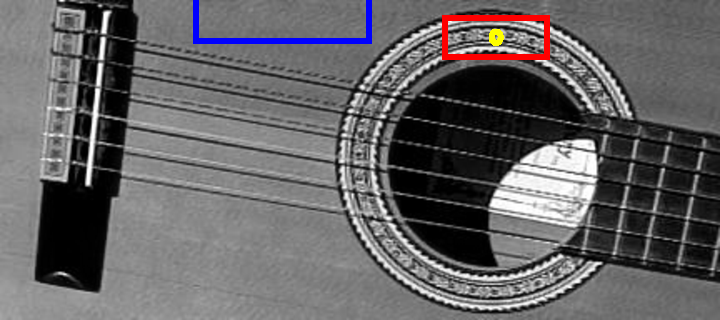
\includegraphics[width=0.2\textwidth]{motionNoiseGaussian/guitar.pdf} &
\includegraphics[width=0.2\textwidth]{motionNoiseGaussian/imageNoiseHistogram.eps} &
\includegraphics[width=0.2\textwidth]{motionNoiseGaussian/motionNoiseHistogram.eps} &
\includegraphics[width=0.2\textwidth]{motionNoiseGaussian/crossCorrelation.eps} \\
(a) Frame from Video & (b) Intensity Noise & (c) Image Noise  & (d) Cross correlation\\
& (Intensity Domain) & (Phase Domain) & \\
\end{tabular}
\caption{We demonstrate that on a real video of a guitar (a) that the noise in intensities (b) and motion noise (c) are approximately Gaussian. The intensity noise ($\sigma = 0.02$) was computed by assuming that the region in blue was spatially constant. Once computed, the regions of high amplitude to noise ratios (>100), such as the one in red were chosen to estimate the motion noise (c, $\sigma=0.02$). This provides some evidence that our model is reasonable. However, the auto correlation shows some correlations, especially in the low frequencies. If this is noise, it shows a problem in our model}
\label{fig:motionNoise}
\end{figure}

\paragraph{Spatial Averaging}
To analyze the non stationary image noise, we consider the problem of estimating the mean of Gaussian-distributed random variables with the same mean and known, but varying variances from a weighted average of the random variables. For random variables $X_i$ with variances $\frac{\sigma^2}{A_i^2}$, their weighted average $\frac{\sum_i w_iX_i}{\sum_i w_i}$ has variance
\beq  V_w = \frac{\sigma^2}{(\sum_i w_i)^2} \left(\sum_i\frac{w_i^2}{A_i^2}\right)\eeq
We can use differential calculs to compute the partial derivatives
\beq \frac{\partial V_w}{\partial w_j} = \frac{\sigma^2}{(\sum_i w_i)^3}\left(\sum_i \frac{2 w_i w_j}{A_j^2}-2\frac{w_i^2}{A_i^2}\right)\eeq
A zero of this system and a stationary point of the variance as a function of the weights is $w_i = A_i^2$. For two variables, it is easy to show that this is a local minima. For large amplitudes $A$, image noise can be approximated by Gaussian noise with variance proportional $\frac{1}{A^2}$. As a result, we propose that any weighted average of the image noise be weighted by the square of the amplitudes. This is different than what we did in our SIGGRAPH paper.

\subsection{No Large Motion Assumption}
We assume that there are no large motions, so that both the image and motion noises are stationary in time. This allows us to perform Weiner filtering on the phase variation signal for each point. Traditional Weiner filtering requires that we know the second order statistics of the signal and noise. Since we do not really know these things, instead we make the assumption that the signal $d[n]$ is narrowband, while the noise $v[n]$ is broadband. and that the noise is decorrlated in time for lags greater than $k_0$. Then, we can use Weiner filtering in a noise cancelation framework. The input noisy signal is then $x[n]:=d[n]+v[n]$. 

As before, we assume our noise is Gaussian, so that the linear MMSE is optimal. Our error function is $d[n]+v[n]-y[n]$ where $y[n]$ is a convolution of $w[n]$, the filter coefficients and a delayed version of the input signal $d[n-k_0]+v[n-k_0]$. Then, the objective is to minimize
\beq \E[(d[n]+v[n]-y[n])^2]\eeq
with respect to $w[n]$. We require that $k_0$ satisfy
\beq \tau_n < k_0 < \tau_s\eeq
where $\tau_n$ is the number of samples for the noise to decorrelate and $\tau_s$ is the number of samples for the signal to decorrelate.
 In \cite{hayes2009statistical}(p. 497), with our assumptions, this is shown to be equivalent to minimizing
\beq E[v[n]^2] + E[(d[n]-y[n])^2]\eeq
Therefore, this framework will allow us to estimate $d[n]$. Again, in \cite{hayes2009statistical}(p. 498), the optimal values of $w$ for a FIR $w$ are given by 
\beq \left(\begin{array}{cccc}
R_x[0] & R_x[1] & \ldots & R_x[n] \\
R_x[1] & R_x[0] & \ldots & R_x[n-1] \\
\vdots & \vdots & & \vdots \\
R_x[n] & R_x[n-1] & & R_x[0] \\
\end{array}\right)
\left(\begin{array}{c}
w[0]\\
w[1]\\
\vdots\\
w[n]\end{array}\right)
 = \left(\begin{array}{c}
R_x[k_0]\\
R_x[k_0+1]\\
\vdots\\
R_x[k_0+n]\\
\end{array}\right)\eeq
We can estimate the auto correlation function empirically from the temporal phase signal. We can also make the assumption that it doesn't vary too much in space and further improve our estimation by performing a amplitude squared weighted blur as discussed in Section 3.2. From this, we can compute the optimal filter coefficients and then perform temporal filtering. 



\begin{figure}
\begin{tabular}{ccc}
\includegraphics[width=0.3\textwidth]{adaptiveFilterExplore10/timeDomain.eps} &
\includegraphics[width=0.3\textwidth]{adaptiveFilterExplore10/freqDomain.eps} &
\includegraphics[width=0.3\textwidth]{adaptiveFilterExplore10/impulseResponse.eps} \\
(a) Time domain & (b) Frequency Domain  & (c) Filter Coefficients\\
\end{tabular}
\caption{In (a-c), we show our denoising method as applied to a sum of very narrowband signal with 1000 samples in time. The noisy signal is several sinusoids of different frequencies summed together with additive Gaussian white noise.}
\end{figure}

We can turn the filter into an adaptive filter to handle certain forms of non-stationarity.

For now, we do this filtering independently on every level of the pyramid.
\section{Results}
\paragraph{Synthetic Videos} In Fig.~\ref{fig:teaser}, we tried our technique on a video fo a synthetic oscillting disk. We did this by applying our temporal filtering to the phase signal of every level of the pyramid independently. The \href{http://people.csail.mit.edu/nwadhwa/writeups/MotionHDR/phaseModel01a/vidDomainComparison.mp4}{Final Results} and the result on the phase signals is shown here: \\
\begin{tabular}{ccccccccccc}
Level & 
\href{http://people.csail.mit.edu/nwadhwa/writeups/MotionHDR/phaseModel01a/phaseLevel2.mp4}{2} &
\href{http://people.csail.mit.edu/nwadhwa/writeups/MotionHDR/phaseModel01a/phaseLevel3.mp4}{3} &
\href{http://people.csail.mit.edu/nwadhwa/writeups/MotionHDR/phaseModel01a/phaseLevel4.mp4}{4} &
\href{http://people.csail.mit.edu/nwadhwa/writeups/MotionHDR/phaseModel01a/phaseLevel5.mp4}{5} &
\href{http://people.csail.mit.edu/nwadhwa/writeups/MotionHDR/phaseModel01a/phaseLevel6.mp4}{6} &
\href{http://people.csail.mit.edu/nwadhwa/writeups/MotionHDR/phaseModel01a/phaseLevel7.mp4}{7} &
\href{http://people.csail.mit.edu/nwadhwa/writeups/MotionHDR/phaseModel01a/phaseLevel8.mp4}{8} &
\href{http://people.csail.mit.edu/nwadhwa/writeups/MotionHDR/phaseModel01a/phaseLevel9.mp4}{9} &
\href{http://people.csail.mit.edu/nwadhwa/writeups/MotionHDR/phaseModel01a/phaseLevel10.mp4}{10} &
\href{http://people.csail.mit.edu/nwadhwa/writeups/MotionHDR/phaseModel01a/phaseLevel11.mp4}{11} \\
\end{tabular}

\paragraph{Natural Videos} We use our optimal filter in time on a few sequences where we expect narrowband signals (guitar, pipe, column, car engine, throat). We boost our estimate of the auto correlation functions by averaging spatially and also post process the phase signal by an amplitude weighted blur. These spatial steps are motivated by Section 3.2, but are somewhat ad hoc and in the future, it will be good to explicitly include the assumption of spatial coherence of the signal. \\
\begin{tabular}{cccc}
\href{http://people.csail.mit.edu/nwadhwa/writeups/MotionHDR/phaseModel01a/comparison-car_engine.mp4}{Car Engine} &
\href{http://people.csail.mit.edu/nwadhwa/writeups/MotionHDR/phaseModel01a/comparison-guitar.mp4}{Guitar} &
\href{http://people.csail.mit.edu/nwadhwa/writeups/MotionHDR/phaseModel01a/comparison-pipe.mp4}{Pipe} &
\href{http://people.csail.mit.edu/nwadhwa/writeups/MotionHDR/phaseModel01a/comparison-throat.mp4}{Throat}\\
\end{tabular}


\section{Discussion}
Our results are not quite as good as the manually tuned narrowband filter, but they are usually better than no filtering, except when the noise level is already quite low such as in the car engine and pipe sequences. We perform worse than narrowband filters because we restrict our automatically detected fitler to be only 60 taps in the natural videos and ten taps in the synthetic video. This is in contrast to the narrowband filters which are implemented using recursive IIR filters. In addition, our assumption that the decorellation time is long for signal is a weaker assumption than assuming that the signal is narrowband. If we were able to integrate the latter assumption into our framework, we might more closely match the results from narrowband filtering. 

\bibliography{references.bib}
\bibliographystyle{plain}

\end{document}